% ----------------------------------------------------------
\chapter{FUNDAMENTAÇÃO TEÓRICA}\label{cap:desenvolvimento}

Para obter resultados de um trabalho é necessário entender o problema, seus componentes, as ferramentas à disposição e saber unir todos os pontos. A primeira parte da fundamentação teórica serve para criar uma base para o entendimento dos componentes: sistema de refrigeração e compressor linear. A segunda parte, e último tópico, explica o método de resolução numérico.

\section{SISTEMAS DE REFRIGERAÇÃO}
% ----------------------------------------------------------

Refrigeradores domésticos geralmente utilizam o ciclo de compressão de vapor com um gás refrigerante, por exemplo, R-134a, que permanece confinado no sistema. O ciclo padrão de compressão é representado na Figura \ref{fig:Fig_1}, onde é possível identificar os seus quatro componentes básicos: condensador, dispositivo de expansão, evaporador e compressor.

\begin{figure}[htb]
	\caption{\label{fig:Fig_1}Ciclo padrão de refrigeração por compressão de vapor.}
	\begin{center}
		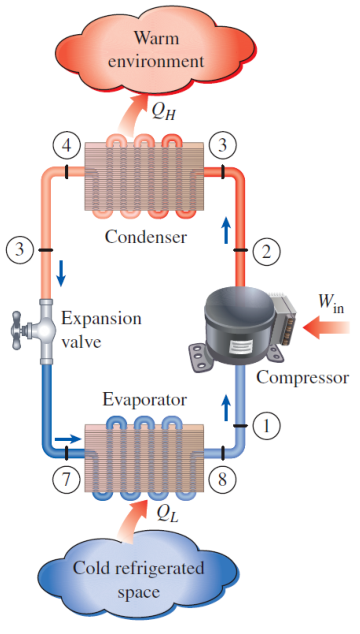
\includegraphics[scale=0.65]{images/refrigerador.png}
	\end{center}
	\fonte{Çengel e Boles (2005)}
\end{figure}

 No ciclo padrão de compressão de vapor ilustrado na Figura \ref{fig:Fig_1}, um fluido na fase gasosa a baixa pressão entra no compressor, que o comprime e superaquece. Em seguida, o fluido de trabalho, a alta temperatura e pressão, passa por um condensador, onde troca calor com o ambiente, vindo a condensar. Após a condensação, o fluido entra num dispositivo de expansão, onde sua pressão e temperatura são reduzidas. Após a expansão, o fluido bifásico passa pelo evaporador, onde absorve calor do espaço refrigerado. Por fim, o fluido retorna para o compressor, onde o ciclo se reinicia.

\section{COMPRESSOR LINEAR}

Normalmente, os compressores de refrigeradores domésticos são alternativos, os quais são classificados como compressores de deslocamento positivo por proporcionarem um aumento de pressão do gás de trabalho a partir da diminuição do seu volume. A câmara de compressão é formada por um conjunto pistão-cilindro, sendo que o movimento alternativo do pistão é geralmente realizado por um sistema biela-manivela. O funcionamento dos compressores lineares é bastante similar. Entretanto, o movimento alternativo do pistão é realizado por um motor linear..
De acordo com Oliveira (2014) é possível encontrar quatro componentes básicos em um compressor linear (Figura \ref{fig:Fig_2}): bobina elétrica, magneto, pistão e molas. A partir de uma tensão elétrica oscilante, a bobina gera um campo eletromagnético variável que exerce uma força sobre o magneto, ocasionando a movimentação conjunta do magneto e do pistão, que estão acoplados. O pistão se move dentro do cilindro e realiza a compressão e expansão do fluido de trabalho. As molas são responsáveis por armazenar energia cinética para que o sistema possa trabalhar em ressonância.


\begin{figure}[htb]
	\caption{\label{fig:Fig_2}Esquemático básico de um compressor linear.}
	\begin{center}
		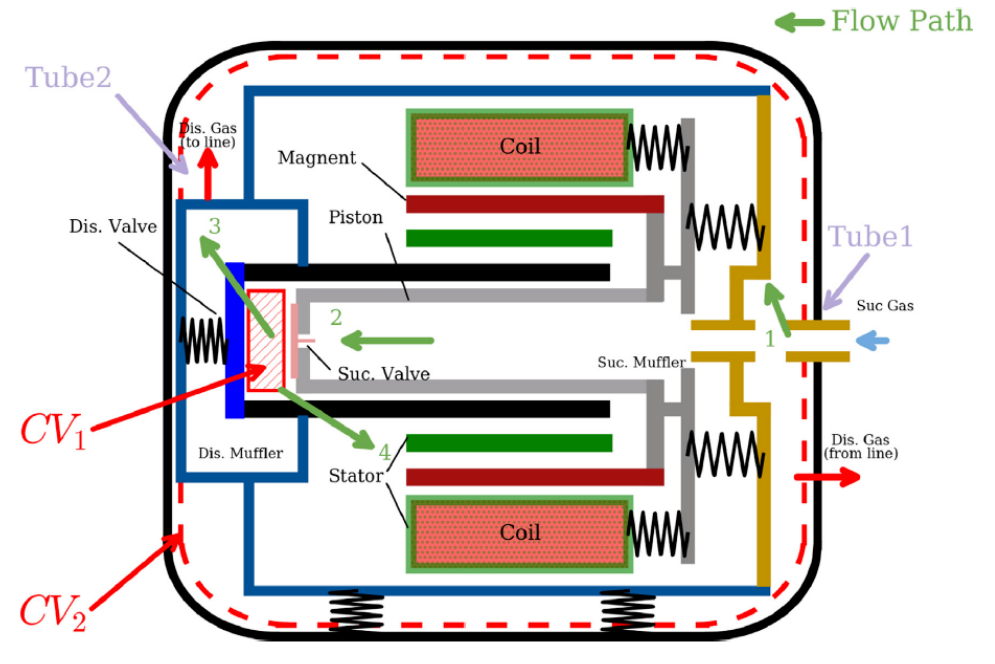
\includegraphics[scale=0.50]{images/compressor.png}
	\end{center}
	\fonte{Zhang et al. (2020)}
\end{figure}

Ainda analisando a Figura \ref{fig:Fig_2}, o caminho percorrido pelo fluido pode ser indicado pelas setas.O fluido de trabalho entra na carcaça do compressor, a baixa pressão, passa por dentro do pistão e é succionada para dentro da câmara de compressão pela válvula de sucção. A válvula de sucção é dita automática, pois abre e fecha de acordo com as diferenças de pressão entre a câmara de compressão e o ambiente interno do compressor. Com o fluido na câmara de compressão e a válvula de sucção fechada o fluido é comprimido durante o movimento ascendente do pistão. A compressão acontece até que a pressão dentro da câmara de compressão seja levemente superior à pressão de descarga, o que ocasiona a abertura da válvula de descarga e a liberação do gás para a linha de descarga.



\section{MÉTODO RUNGE KUTTA DE 4ª ORDEM}

O método de Runge-Kutta (RK) é utilizado para resolver equações diferenciais ordinárias (EDO) com problema de valor inicial (PVI). Assim como Zhang et al. (2020a), este trabalho adotará o método de RK de quarta ordem para resolver as equações governantes do problema. Como as equações descritas neste trabalho são de segunda ordem, foi necessário transformá-las em um sistema de duas equações de primeira ordem para aplicar o método. Sendo assim, a explicação se restringe a uma EDO genérica de primeira ordem.
Seja y'a derivada primeira de y, onde y é uma função de t.Valores iniciais de y' e y são conhecidos e mostrados nas Equações \ref{eq:y_linha} e \ref{eq:y_comum}:



\begin{equation}\label{eq:y_linha}
y' = f(t,y),
\end{equation}


\begin{equation}\label{eq:y_comum}
y(t_0)=y_0,
\end{equation}


A solução que o método Runge-Kutta propõe para a EDO a cada intervalo discreto de tempo é dado pelas Equações \ref{eq:y} e \ref{eq:t}:




\begin{equation}\label{eq:y}
y_{n+1}=y_n+ \frac{h}{6}(K1+2K2+2K3+K4),
\end{equation}


\begin{equation}\label{eq:t}
t_{n+1}=t_n+h,
\end{equation}
onde a letra h é o passo de tempo do método, e n um número inteiro que representa o índice relacionado a um determinado instante de tempo. As funções K1, K2, K3 e K4 são definidos nas Equações \ref{eq:k1}, \ref{eq:k2}, \ref{eq:k3} e \ref{eq:k4}:


\begin{equation}\label{eq:k1}
K1=f(t_n,y_n),
\end{equation}

\begin{equation}\label{eq:k2}
K2=f(t_n+ \frac{h}{2},y_n+\frac{h}{2}K1),
\end{equation}

\begin{equation}\label{eq:k3}
K3=f(t_n+ \frac{h}{2},y_n+\frac{h}{2}K2),
\end{equation}

\begin{equation}\label{eq:k4}
K4 = f(t_n + h, y_n + hK3 ).
\end{equation}


